\section{Apache Hadoop\textsuperscript{\textregistered} Framework}
\label{sec:theory_hadoop}
\noindent
Apache Hadoop ist ein etabliertes Java-Framework zur verteilten Speicherung und Verarbeitung von Daten. Durch die parallele Ausführung von Algorithmen eignet sich ein Hadoop-Cluster für rechenaufwendige Datenanalysen. Ein primäres Paradigma ist das Konzept der \textit{Datenlokalität}. Die auszuführenden Programme werden auf die Knoten verteilt, auf welchen auch die Daten liegen. Ressourcenintensive Datentransporte sollen weitgehend vermieden werden.\cite[S. 20 ff.]{big_data_praxis}\\ 
Das Framework ist für die Ausführung auf Standardhardware konzeptioniert. Es wird also keine verhältnismäßig teure Spezialhardware benötigt. Das Cluster besteht aus vielen einzelnen Knoten mit Standardhardware, welche im Verhältnis zu Spezialhardware günstiger und leicht ersetzbar ist. Der Ausfall einzelner Knoten ist die Regel und wird bei der Datenhaltung entsprechend berücksichtigt. \\

\noindent
Das Apache Hadoop\textsuperscript{\textregistered} selbst besteht aus mehreren Komponenten, welche spezifische Aufgaben übernehmen. Abbildung \ref{fig:hadoop_framework_structure} stellt eine grobe Skizzierung der Komponentenlandschaft von Apache Hadoop dar.\footnote{In der Abbildung \ref{fig:hadoop_framework_structure} werden Logos der einzelnen Apache Projekte verwendet. Diese sind Handelsmarken der \textit{Apache Source Foundation} (siehe \url{https://www.apache.org/}). In Kapitel \ref{sec:licencing_issues} im Anhang werden die Logos und deren Herkunft nochmals aufgelistet.}\\

\begin{figure}[ht]
  \centering
  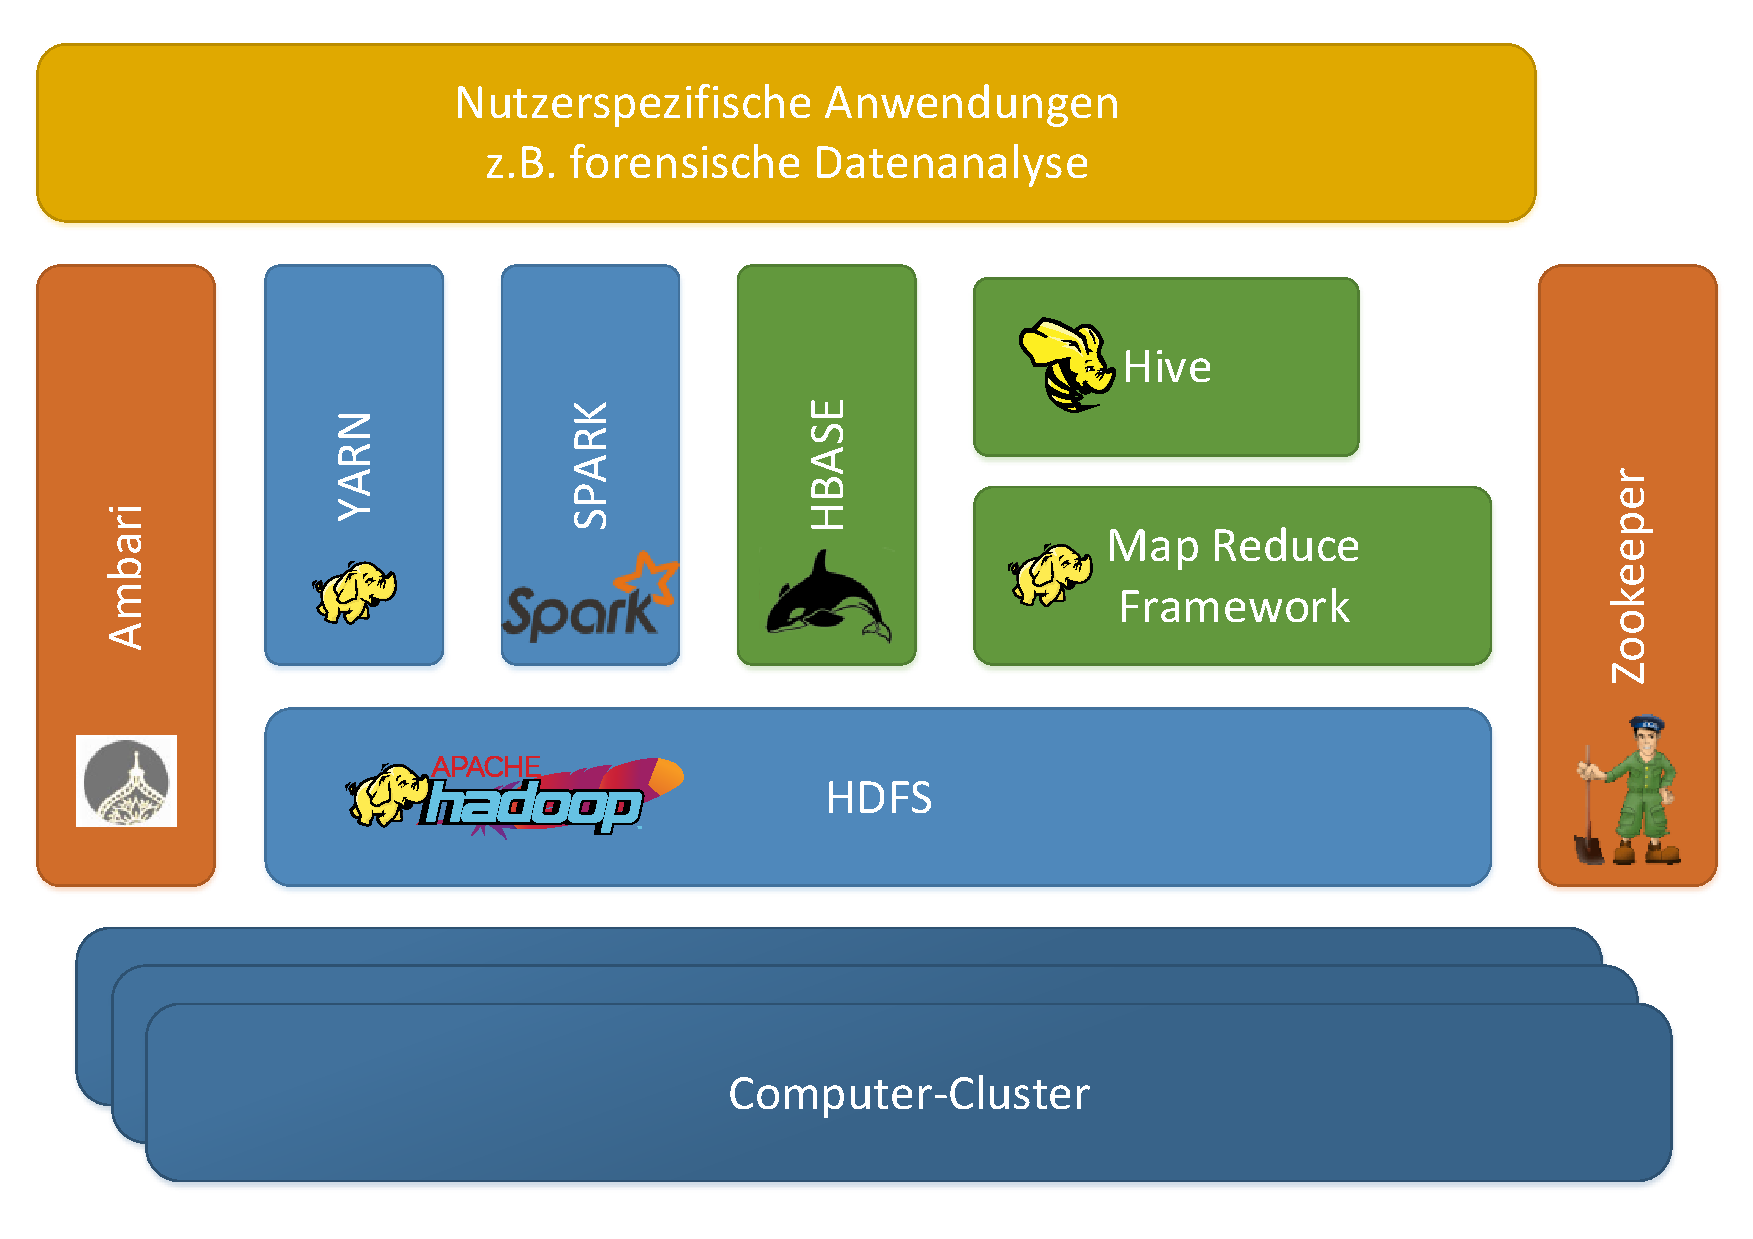
\includegraphics[width=\textwidth]{./resource/hadoop_framework_structure.pdf}
  \caption{Apache Hadoop Ökosystem (Vgl. \cite{big_data_praxis},\cite{expert_hadoop_admin}. Siehe Kapitel \ref{sec:licencing_issues})}
  \label{fig:hadoop_framework_structure}
\end{figure}

\noindent
Die Basis bildet das verteilte Dateisystem \textit{Hadoop Distributed File System (HDFS)}, welches die Daten redundant auf allen Knoten des Computer-Clusters speichert. Hierbei besteht das Computer-Cluster selbst aus mehreren Knoten, auf welchen vorzugsweise ein Linux-Betriebsystem, wie beispielsweise CentOS, arbeitet.\\
Der Ressourcenmanager \textit{YARN (Yet Another Resource Negotiator)} ist für die Verteilung und Bereitstellung von verfügbarer Rechenleistung verantwortlich.\\ 
Die dritte Komponente ist das \textit{Hadoop\textsuperscript{\textregistered} Map-Reduce Framework}. Hadoop Map-Reduce kann zur Datenverarbeitung genutzt werden. Hierbei werden Algorithmen parallel auf den Knoten prozessiert und die Ergebnisse im Anschluss zusammengetragen. Die einzelnen Zwischenergebnisse werden alle im HDFS abgelegt.\footnote{Sogenannte Map-Reduce Jobs bildeten in den Anfängen von Hadoop den primären Weg, Daten verteilt zu verarbeiten. Mittlerweile wurde diese Art der Datenverarbeitung in den Hintergrund verdrängt, da andere Projekte, wie beispielsweise Apache Spark, die Daten schneller verarbeiten können oder andere Ansätze zur Verarbeitung nutzen. Dies ist beispielsweise auch der Grund, weshalb Hadoop Map-Reduce in dieser Masterthesis nicht explizit verwendet wird.} \\

\noindent
Das verteilte Dateisystem HDFS und der Ressourcenmanager YARN bilden den Kern des Hadoop-Clusters. Darauf aufbauend können andere Komponenten die Daten verarbeiten oder spezielle Aufgaben durchführen.\\
So wird beispielsweise in dieser Thesis \textit{Apache Spark\texttrademark\thinspace} bei der Prozessierung und Analyse der Daten genutzt. Der Vorteil von Apache Spark ist eine performante Datenverarbeitung, da einerseits die Daten verteilt verarbeitet werden und andererseits Zwischenergebnisse und temporäre Daten im Arbeitsspeicher der einzelnen Rechenknoten gehalten werden.\footnote{Durch das In-Memory Computing ist Apache Spark deutlich schneller als das bereits vorgestellte Hadoop Map-Reduce.}\\
Desweiteren bietet \textit{Apache Hive\texttrademark\thinspace} eine Möglichkeit Dateien im HDFS mithilfe einer SQL ähnlichen Syntax\footnote{Dem sogenannten HiveQL.} abzufragen. Hierbei nutzt die Komponente wiederum das Map-Reduce Framework von Hadoop. Apache Hive ist jedoch keine reine Datenbank, sondern arbeitet auf den Dateien im HDFS.\\
\textit{Apache HBASE\textsuperscript{\textregistered}} hingegen ist eine spaltenorientierte Key-Value Datenbank. Sie wurde eigens für Apache Hadoop implementiert, 
um große Datenmengen performant zu speichern.\\

\noindent
Das Hadoop-Ökosystem als Ganzes muss auch konfiguriert und überwacht werden. Um die Verfügbarkeit einzelner Instanzen zu gewährleisten und gegebenenfalls redundante Verarbeitungswege anzubieten, wird \textit{Apache ZooKeeper\texttrademark\thinspace} genutzt. Mit ZooKeeper ist es auch möglich Konfigurationen und Änderungen im Cluster zu verteilen. Zum eigentlichen konfigurieren und überwachen des Hadoop-Clusters wird \textit{Apache Ambari\texttrademark\thinspace} genutzt.\\

\noindent
Zusätzlich existieren weitere Projekte im Hadoop-Ökosystem, welche für die forensische Analyseplattform von Verwendung sein können.
Hierzu gehören:
\begin{itemize}
\item \textit{Apache Livy} zur Ausführung von Apache Spark Anwendung über eine REST-Schnittstelle.\footnote{\textit{Representational State Transfer (REST)} bezeichnet ein Programmierparadigma in verteilten Systemen. Hierbei werden Ressourcen über HTTP angefordert, gespeichert und verarbeitet.}
\item \textit{Apache NiFi} ermöglicht das Aufbereiten von Daten und organisiert Datenimporte.
\item \textit{Apache UIMA\texttrademark\thinspace} zur Analyse von unstrukturierten Daten, wie beispielsweise Texte und Mediadateien. \textbf{TODO: Kann UIMA überhaupt in Hadoop eingesetzt werden.}
\item \textit{Apache Accumulo\textsuperscript{\textregistered}} als Alternative zu Apache HBASE?
\end{itemize} 

\noindent
Prinzipiell sind viele Komponenten unabhängig voneinander. So kann ein HDFS ausschließlich zur Datenhaltung aufgebaut werden, ohne eine Komponente zur Datenverarbeitung verwenden zu müssen. Umgekehrt lassen sich Komponenten zur Datenverarbeitung, wie Apache Spark, auch ohne das HDFS und YARN nutzen und könnten damit auch in andere Umgebungen integriert werden. Die einzelnen Komponenten entfalten jedoch gerade durch die Kombination miteinander ihre Potential zur performanten Datenanalyse.\\

\noindent
Es gibt einige Unternehmen, die sich speziell daruf spezialisiert haben dieses Apache Hadoop Ökosystem und weiter noch nicht erwähnte Komponenten zu einzelnen Analyseplattformen zusammenzufassen. Sie bieten hierfür entsprechender kostenpflichtiger Support, wobei diese Plattformen im reinen Betriebe kostenfrei sind. So wird im Praxisteil der Masterthesis beispielsweise die \textit{Hortonworks Data Platform (HDP)} des Unternehmes \textit{Hortonworks} genutzt.


\section{Apache Hadoop HDFS}
\label{sec:theory_hdfs}
Das Hadoop Distributed Filesystem (HDFS) ist ein verteiltes Dateisystem, welches die Grundlage zu Speicherung von Daten im Hadoop-Ökosystem bietet. Nachfolgende Zwecke soll es erfüllen.\\
Es soll ausfallsicher sein. In der Standardkonfiguration wird jede Datei dreifach auf unterschiedlichen physikalischen Knoten gespeichert. Damit kann selbt bei einem Ausfall von zwei Knoten immer noch auf die Datei zugegriffen werden. Darüber hinaus verteilt das HDFS die Dateien automatisch und regeneriert sich selbst nach Ausfällen von Knoten. In großen Computer-Clustern mit mehreren hunderten Knoten ist ein Ausfall eines Knoten kein Sonderfall sondern die Regel. Daher muss sich das HDFS selbst heilen können, um auch ohne manuelle Administration weiter verfügbar zu sein.\\
Das HDFS (und auch Hadoop im allgemeinen) soll horizontal skalierbar sein. Wird mehr Speicher benötigt, sollen einfach noch Knoten hinzugefügt werden können.\\
Das HDFS ist auf hohen Datendurchsatz und die Speicherung großer Datenmengen ausgelegt.
So können einzelne Dateien mehrere Gigabyte bis hin zu Terrabyte groß seind und es können mehrere Millionen Dateien im HDFS gespeichert werden. Die Optimierung auf einen möglichst hohen Datendurchsatz geht mit einer schlechteren Reaktionszeit im Vergleich zu herkömlichen Dateisystemen einher.\\
Das Prinzip \textit{Write-once-Read-many} wird im HDFS implementiert. Wenn Daten einmal geschrieben wurden, dann werden sie normalerweise nicht mehr geändert. Dies ermöglicht ein einfacheres Koherenzmodell. Dies fördert den Lesedurchsatz indem die Unterstützung der Modifikation von Daten stark eingechränkt wird. Ein wahlfreies Schreiben in eine existierende Datei wird beispielsweise nicht unterstützt. Änderungen an Daten, welche von Algorithmen vorgenommen werden, resultieren in neuen Datensätzen.\\
Darüber hinaus gilt das Prinzip der Datenlokalität. Algorithmen werden dort ausgeführt, wo die Daten liegen, um das Verschieben von Daten über das Netzwerk zu vermeiden.\cite{hdfs_architecture}\\

\noindent
Der Aufbau eines HDFS bildet eine Master-Slave Architektur aus \textit{NameNodes} und \textit{DateNodes}. Der NameNode is einmalig im verteilten System vorhanden und enthält alle Metainformationen zu den Dateien. Eine Datei selbst wird in ein oder mehrere Blöcke aufgeteilt und auf mehreren DateNodes gespeichert. Der NameNode organisiert diese Speicherung und bestimmt, wo welche Daten persistiert werden. Über den NameNode selbst fließen aber keine Rohdaten von Dateiinhalten. Auf Dateisystemebene ist das HDFS wie gängige Dateisystem hierarchisch organisiert. Jede Datei wird über einen absoluten Pfad eindeutig bestimmt und erhält entsprechende Metadaten, wie Dateirechte und Zeitstempel.  \\

\noindent
Abbildung \ref{fig:hdfs_cluster_architecture} verdeutlicht die Struktur im HDFS. Angenommen es soll die Datei \path{/home/foo.txt} gespeichert werden. Dies kann mit dem Terminalprogramm \textit{hdfs} durchgeführt. Das Programm selbst ist hier der HDFS-Client und hat Zugang zum Hadoop-Cluster. Der HDFS-Client speichert zuerst die Metadaten der Datei auf dem Name Node. Der Name Node bekommt die Größe der Datei auch mit und entscheidet dann, in viele Blöcke sie unterteilt werden soll. Darauf hin ermittelt für jeden einzelnen Block, auf welchen Date Nodes dieser Block gespeichert werden soll. Diese Blockaufteilung und die Zuordnung zuden Date Nodes werden an den HDFS-Client zurückgeschickt. Dieser übermittelt die Blöcke an einen der Data Nodes. Sobald der erste Data Node einen Block hat, sorgt er dafür die Blöcke an die anderen Data Nodes weiterzuleiten. Die Data Nodes selbst stehen auch in Kontakt zum Name Node und reporten ihren Zustand und die momentan gespeicherten Blöcke. Der Name Node bekommt darüber auch mit, wenn ein Data Node ausfällt.

\begin{figure}[ht]
  \centering
  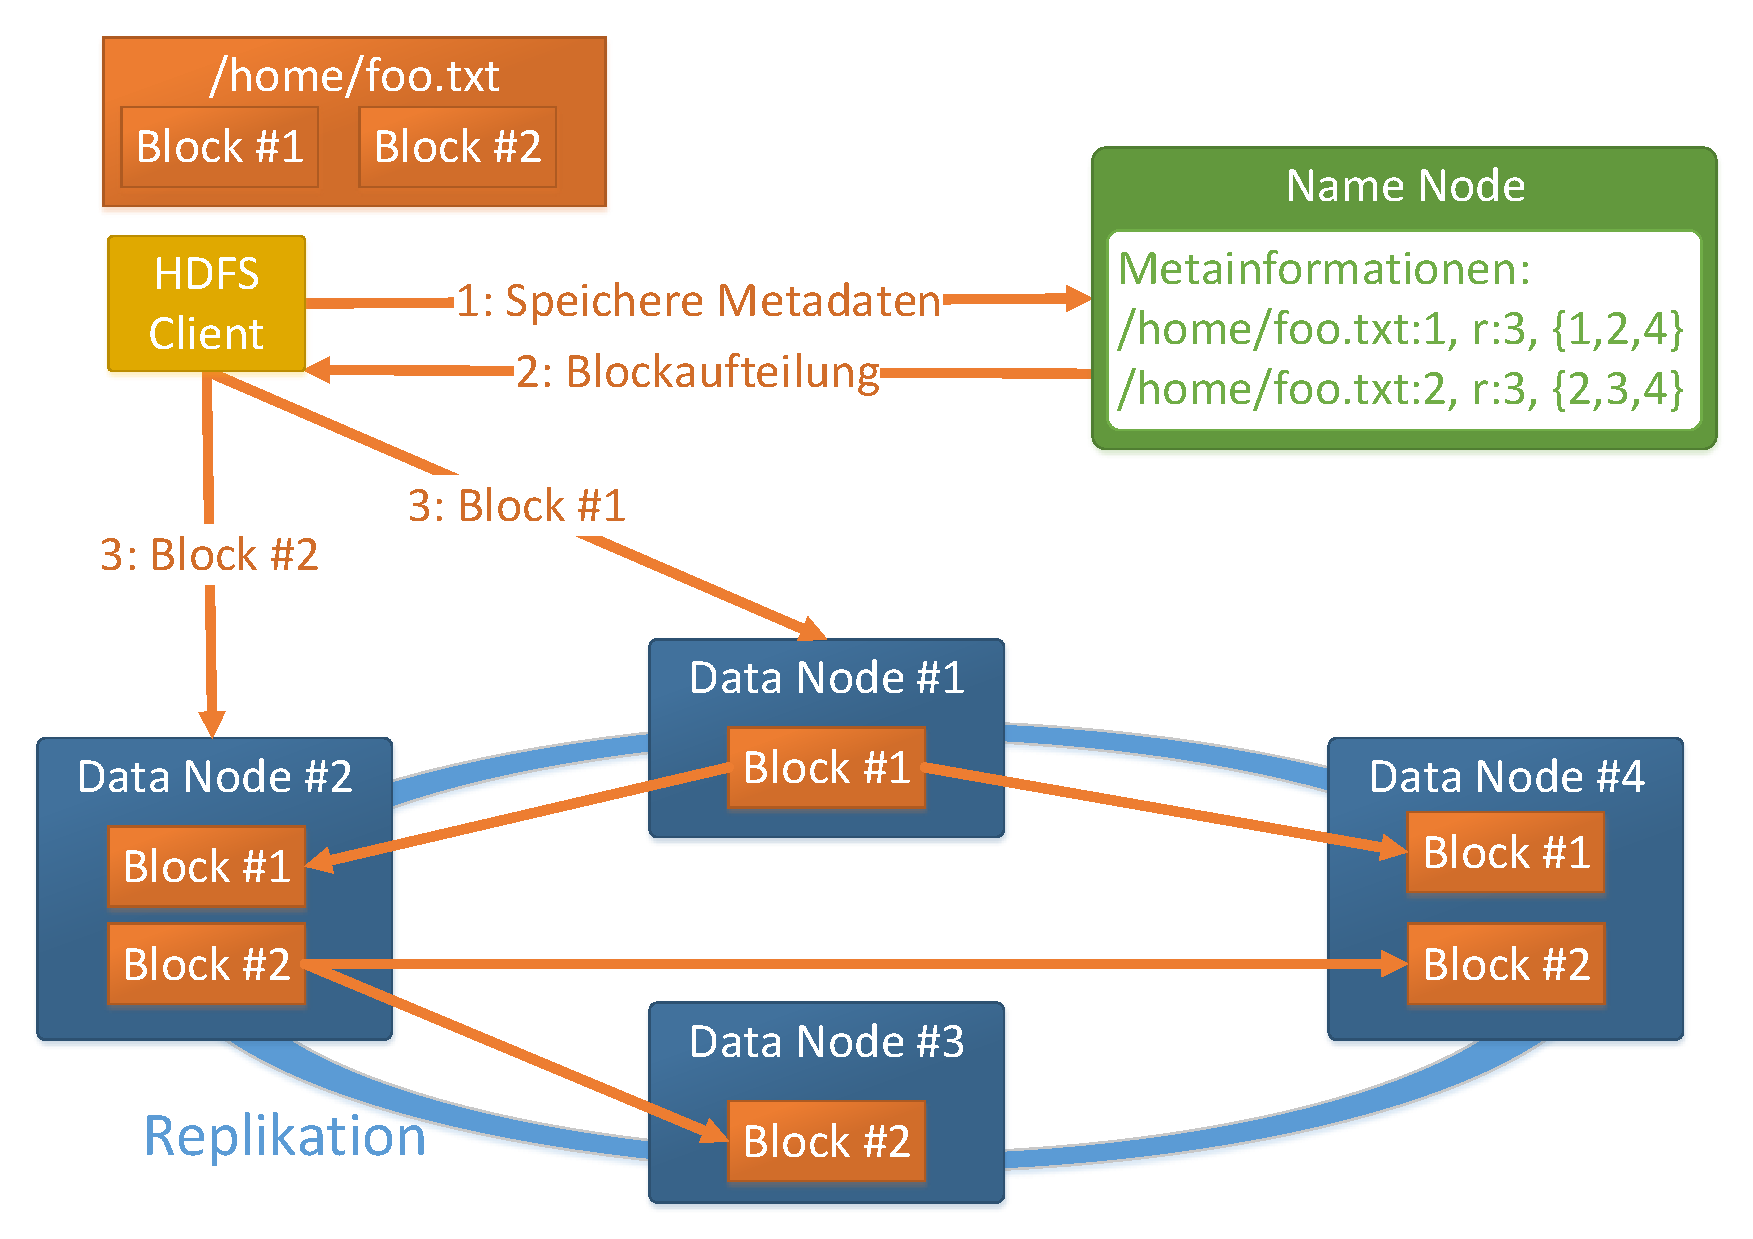
\includegraphics[width=\textwidth]{./resource/hdfs_cluster_architecture.pdf}
  \caption{HDFS - Datenspeicherung im Verbund (Vgl. \cite{hdfs_architecture},\cite{expert_hadoop_admin})}
  \label{fig:hdfs_cluster_architecture}
\end{figure}

\noindent
Ein Block hat in der Standardkonfiguration 128 MB. Er kann aber auch bis zu 512 MB Größe konfiguriert werden. Dies wirft die Frage auf, ob das HDFS gerade für sehr kleine Dateien, wie sie bei der Analyse von Datenträgern auch vorkommen, nicht zu viel Speicher verschwendet. \\
Hierbei wird der gleiche Block immer in unterschiedlichen Data Nodes angelegt. Es ist nicht erlaubt den gleichen Block mehrmals im gleichen Data Node zu replizieren. Daher ist die Anzahl der Replikationen auch kleiner gleich der Anzahl Data Nodes im System.

\noindent
Wichtig hierbei ist auch, dass im Produktivsystem auf jedem physikalischen Knoten auch nur ein DataNode oder ein NameNode läuft. Denn würden beispielsweise mehrere DateNodes auf dem gleichen physikalischen Knoten laufen, so wäre bei einem Ausfall nicht mir garantiert, dass die Dateiinhalte auch noch auf mindestens zweie anderen Knoten laufen. Denn der Replikationsmechanismus im HDFS kann nicht erkennen, ob jeder Knoten physikalisch unabhängig arbeitet. Allerdings hat Hadoop eine sogenannte \textit{Rack-Awareness}. So ist es möglich zu bestimmen, welche physikalischen Server in einem gemeinsamen Rack laufen. Abhängig davon, versucht das HDFS die Daten teilweise im selben Rack redundant zu speichern aber auch einige Replikationen außerhalb des Racks anzulegen. So kann auch der Ausfall eines Racks im Notfall kompensiert werden.\\
In Testumgebungen ist aber schön möglich sogar NameNode und mehrere DateNodes auf einem Knoten laufen zu lassen. Allerdings greifen die Mechanismen für eine Toleranz gegenüber Hardwareausfällen dann nicht mehr.\\

\noindent
Wie oben ersichtlich, ist der Name Node die Schlüsselstelle im HDFS-Cluster. Dieser bildet einen \textit{Single Point of Failure}. Denn bei einem Ausfall wäre das HDFS nicht mehr einsatzbereit. Es existiert ein sogenannter \textit{Secondary Name Node}. Dieser erhält die Metainformationen und erstellt daraus regelmäßig Checkpoints. Der Name Node hält die Metainformationen im Arbeitsspeicher. Es existiert aber auch eine Datei \textit{FsImage} und ein \textit{EditLog}, welche persistent auf der Festplatte gespeichert sind. Das FsImage selbst beschreibt einen Zustand der Dateisystemmetainformationen zu einem gewissen Zeitpunkt. Im EditLog befinden sich alle Änderungen seit dem letzten Checkpoint bis zum aktuellen Zeitpunkt. Der Secondary Name Node erstellt aus dem FsImage und dem EditLog regelmäßig neue Checkpoints, die dann der produktive Name Node bei einem möglichen Neustart wiederverwenden kann. Der \textit{Secondary Name Node} unterstützt also den (First) Name Node, er kann ihn aber nicht ersetzen.\\
Daher ist es möglich auch einen sogenannten \textit{Standby Name Node} zu konfigurieren. Dieser kann einspringen, sobald der erste Name Node ausgefallen ist. Allerdings muss dieser extra konfiguriert werden. Dafür kann aber dann der Secondary Name Node deaktiviert werden.\cite[S. 88]{expert_hadoop_admin}\textbf{ TODO: prüfen ob das wirklich stimmt!}\\

\noindent
Das HDFS selbst kann über mehrere Wege genutzt werden. Es gibt eine Kommandozeilenschnittstelle, die sogenannte \textit{FS Shell}. Es ist möglich über eine Java oder C++ - Schnittstelle Datenzugriff zu erhalten. Oder das Dateissystem kann über eine REST-Schnittstelle via HTTP(S) genutzt werden. Auch das Mounten als \textit{Network File System (NFS)} ist möglich?

\section{Apache Hadoop YARN}
\label{sec:theory_yarn}
YARN ist ein Ressourcenmanager, welcher die verfügbaren Ressourcen innerhalb des Hadoop Clusters organisiert und die Ausführungsreihenfolge von Jobs plant und überwacht. Es gibt einen \textit{Resource Manager}, welcher nur die Ressourcen verwaltet. Auf jedem Knoten, welcher auch Datenverarbeitungen durchführt, ist ein \textit{Node Manager} aktiv. Zuletzt gibt es noch einen \textit{Application Manager} für jeden einzelnen Job, der ausgeführt werden soll. Der Application Manager kontrolliert die Ausführung des Jobs.\\
Abbildung \ref{fig:yarn_cluster_architecture} zeigt die Komponenten von YARN im Cluster.\\

\begin{figure}[ht]
  \centering
  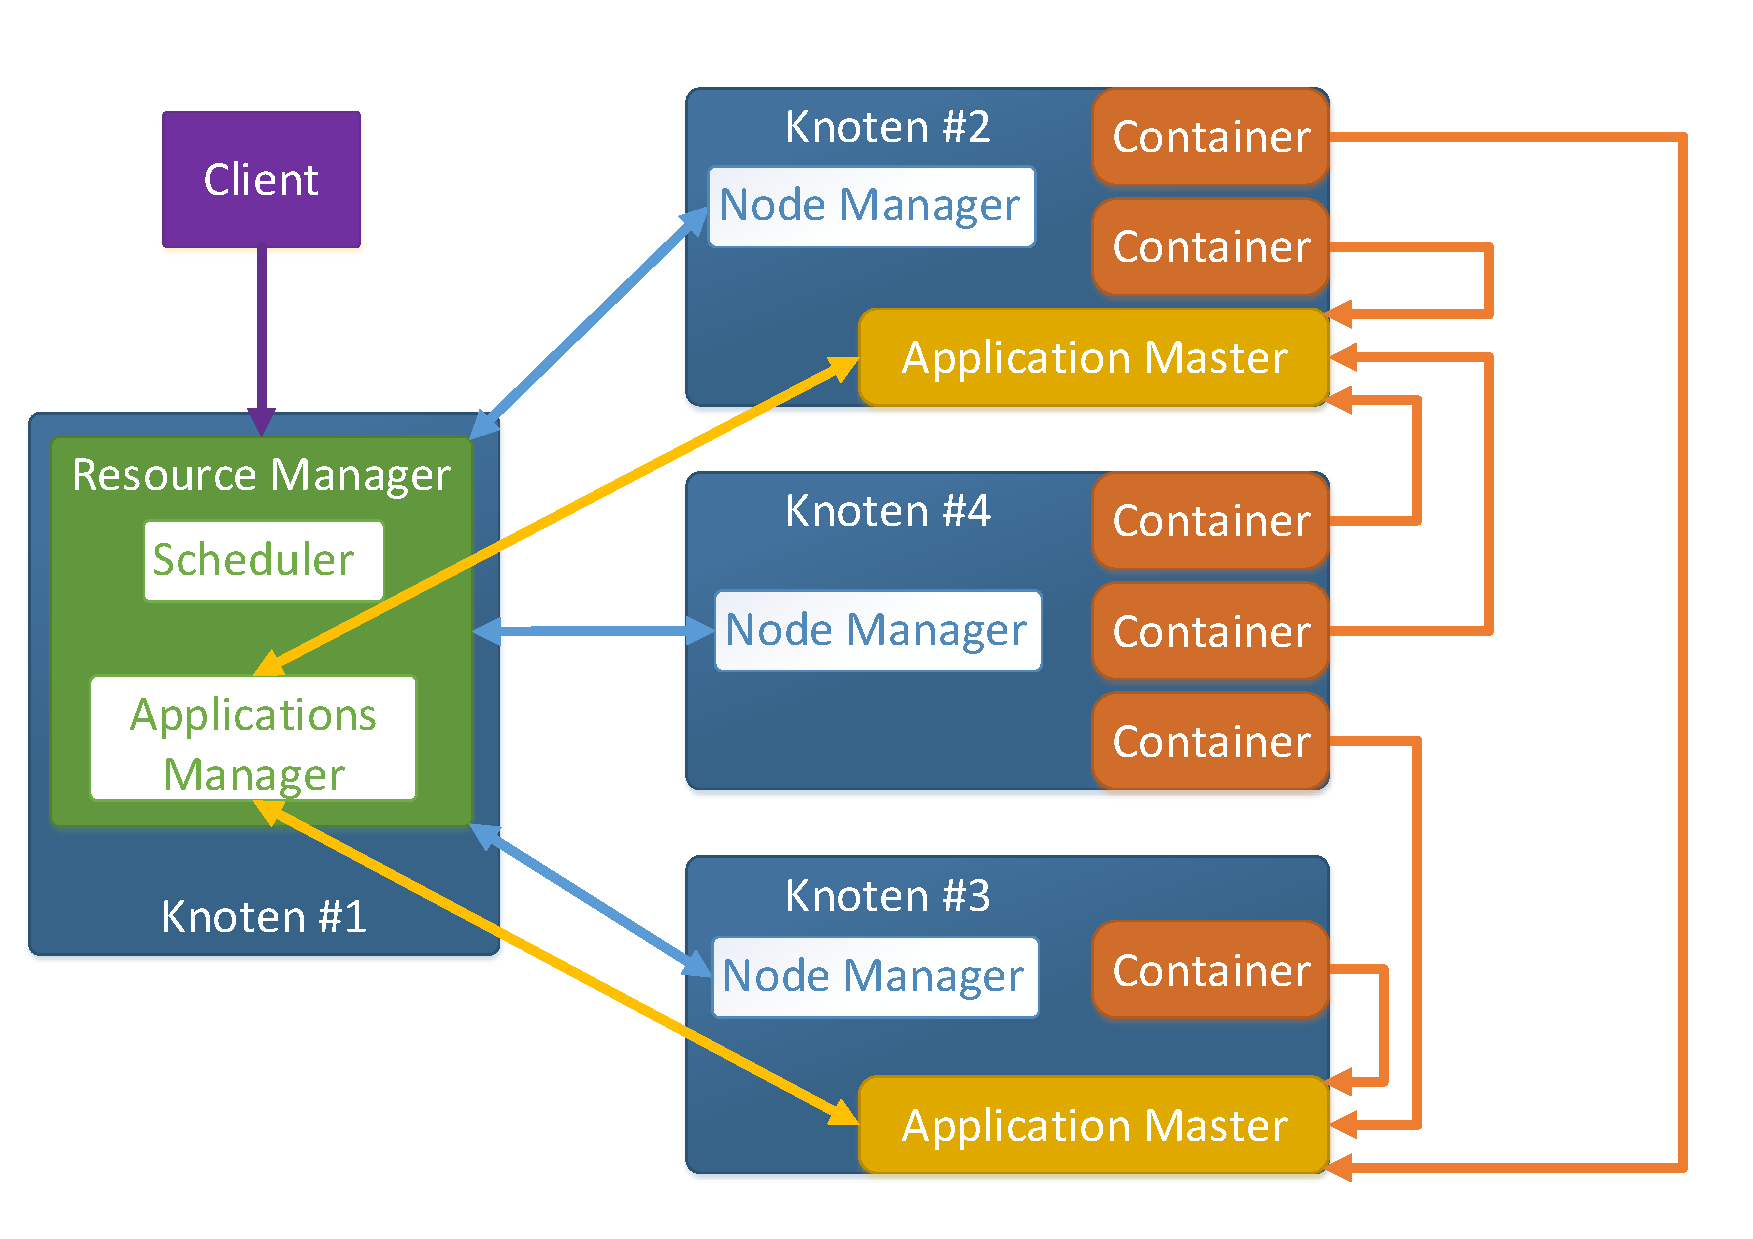
\includegraphics[width=\textwidth]{./resource/yarn_cluster_architecture.pdf}
  \caption{Ressourcenverteilung mit YARN (Vgl. \cite{yarn_architecture},\cite{expert_hadoop_admin})}
  \label{fig:yarn_cluster_architecture}
\end{figure}

\noindent
Ein Job oder eine Anwendung besteht aus mehreren Tasks. Diese Tasks können parallel in mehreren sogenannten Container ausgeführt werden. Ein Container ist eine abstrakte parallele Verarbeitungseinheit, welche bestimmte CPU- und Speicher-Ressourcen enthält. Es können mehrere dieser Container auf einem Knoten innerhalb des Clusters ausgeführt werden. Beispielsweise werden bei einem Knoten mit einer Quad-Core CPU und Hyperthreading (mit insgesamt 8 ausführbaren Threads) bis zu 8 Container erstellt. Bei 32 GB Arbeitsspeicher könnten dann jedem Container 4 GB zugeteilt werden.\footnote{In der Praxis ist es meistens weniger, da entsprechende Ressourcen für das darunter liegende Betriebssystem und YARN selbst reserviert werden.}\\
Derzeit werden für den Container die Anzahl der CPU-Cores (Ausführbare CPU-Threads) und die Größe des nutzbaren Arbeitsspeichers definiert.\cite[S. 48 ff.]{expert_hadoop_admin}\\

\noindent
Wenn nun eine Anwendung über YARN im Cluster ausgeführt werden, soll dann sendet ein Client eine Anfrage an den Resourcen Manager. 
Für jeden auszuführenden Job erstellt der Resource Manager den ersten Container. In diesem Container wird dann der Application Manager gestartet, welcher sich dann im weiteren Verlauf um die Ausführung des Jobs kümmert. Der Resource Manager selbst kennt die Anwendung nicht, noch weiß er wie diese ausgeführt werden. 
Er ist nur dafür zuständig Resourcen zu verteilen.\\ 
Der Application Master hingegen ist sehr spezifisch. Wird zum Beispiel eine Apache Spark Anwendung mit YARN ausgeführt, so ist der Application Master der sogenannte \textit{Spark App Master}. Nachdem nun der Application Master mit im ersten erzeugten Container gestartet wurde, kann dieser wiederum neue Ressourcen beim Resource Manager anfordern. An dieser Stelle zeigt sich der Vorteil von YARN in Kombination mit dem HDFS. Denn bei der Anforderung von Ressourcen gibt der Application Manager an, wieviele Container (inklusive Arbeitsspeicher und CPU) er benötigt. Zusätzlich übermittelt er die Dateiblöcke, welche er aus dem HDFS braucht und an welchen Knoten er welche Container gerne starten würde. So würde der Application Manager 1 auf dem Knoten 2 (siehe Abbildung \ref{fig:yarn_cluster_architecture}) einen Container auf dem Knoten 2 und zwei Container auf dem Knoten 4 mit beispielsweise 1 GB Arbeitsspeicher und 1 Core anfordern. Denn der Application Master weiß, dass dort die benötigten Datenblöcke im HDFS gespeichert sind. Hierbei ist es wichtig zu verstehen, dass die Knoten aus Abbildung \ref{fig:yarn_cluster_architecture} den Data Nodes aus Abbildung \ref{fig:hdfs_cluster_architecture} entsprechen.\footnote{Wobei ein physikalischer Knoten, auf welchem ein Data Node läuft nicht zwingend auch für die Datenverarbeitung mit YARN verwendet werden muss. Beziehend auf das Paradigma der Datenlokalität ist dies aber der Normalfall, dass ein Knoten, welcher Daten persistiert, auch Daten verarbeiten wird.}\\

\noindent
Der Application Master erhält dann die Zustimmung vom Resoure Manager, nachdem der Scheduler die geforderten Resourcen entsprechend eingeteilt hat. Darauf fordert der Application Manager den Node Manager auf den jeweiligen Knoten auf, entsprechende Container zu erstellen.\\
Die einzelnen Node Manager stehen in Kontakt zum Resource Manager und reporten ihm den aktuellen Status des Knoten und dessen Auslastung. \\
Nach der Ausführung der einzelnen Tasks innerhalb der Container und dem Abschluss des Jobs, schickt der Application Manager die Ergebnisse direkt zurück zum Client.\footnote{Hierbei werden die fachlichen Ergebnisse, meistens als Datei im HDFS gespeichert.}. Danach meldet er sich beim Resource Manager ab. Zuletzt kümmert sich der Resource Manager dann über das Freigeben von allokierten Resourcen.\\

\noindent
Ähnlich wie beim Prozessschedulung in ein herkömmlichen Betriebssystem, gibt es auch für YARN unterschiedlicher Algorithmen, die festlegen, in welcher Reihenfolge und Zeitdauer die einzelnen Jobs ausgeführt werden. Bekannte Scheduler sind der \textit{Fair Scheduler} und der \textit{Capacity Scheduler}. Abhängig von der genutzten Plattform/Distribution einzelner Hersteller ist für YARN ein anderer Scheduler konfiguriert. In etlichen Fällen wird der Capacity Scheduler als Standard konfiguriert, da dieser versucht alle Knoten möglichst effizient auszusteuern um den höchstmöglichen Datendurchsatz durch erreichen. Der Fair-Scheduler prüft hingegen, dass jedem Job die gleichen Ressourcen zugeteilt werden, um möglichst alle Jobs parallel bedienen zu können.\textbf{TODO: Scheduling prüfen!}

\noindent
In großen Clustern wird die Prozessierung in mehrere Sub-Cluster mit eigenen Resource Managern aufgeteilt. Diese Struktur wird in der Literatur als \textit{Federaded YARN} beschrieben und soll die Skalierbarkeit von YARN in großen Clustern ermöglichen.

\section{Apache Spark}
\label{sec:theory_spark}

\textit{Apache Spark\texttrademark\thinspace} ist ein Projekt zur verteilten Prozessierung von großen Datenmengen. Mit Apache Spark können verschieden Algorithmen und Verarbeitungsschritte über eine einheitliche Programmierschnittstelle auf gespeicherte Daten  angewendet werden. Spark selbst kümmert sich um die Verteilung, Ausführung und Überwachung der Applikationen zur Datenverarbeitung.\cite[S. 2]{learning_spark}\\
Apache Spark ist mittlerweile schon fast der Standard, wenn es im Hadoop-Umfeld um die Datenverarbeitung geht. Es löst damit auch das ursprünglich verwendete MapReduce-Framework von Hadoop ab, denn Spark
bietet einen enormen Geschwindigkeitsvorteil gegenüber dem MapReduce-Framework. Dies lässt auf einer intelligenten Ausführung einzelner Verarbeitungsschritte und diversen Optimierungen zurückführen.\cite[S. 148 ff.]{expert_hadoop_admin}\\

\noindent
Ein anderer Aspekt sind auch die vielseitigen Einsatzzwecke von Spark. So wird die klassische Datenverarbeitung von statischen Datenmengen\footnote{In diesem Kontext ist das einfache Ausführen einer Anwendung auf eine bereits existierende Datenmenge gemeint, welches am Ende an definiertes Ergebnis liefert.} unterstützt auch die Verarbeitung von dynamischen Datenmengen (Streaming-Data) \footnote{Bei der Datenverarbeitung von Streaming-Data wächst die zu verarbeitende Datenmenge dynamisch and und die ausgeführte Anwendung verarbeitet die neu hinzugekommenen Daten. Ein Beispiel wäre das Filtern von Tweets auf Twitter nach bestimmten Merkmalen, wobei auch neu hinzukommende Tweets bearbeitet werden und nicht nur die Tweets, welche beim Ausführungszeitpunkt der Anwendung bereits existierten.}. Auch die Prozessierung von Graphen-Strukturen und das maschinelle Lernen werden unterstützt.\cite[S. 152]{expert_hadoop_admin}
Darüber hinaus steht es dem Anwender frei, ob er seine Applikationen in Scala, Python oder Java schreibt. Gerade bei den Interpreter-Sprachen Scala und Python gibt es sogar ein Spark-Shell zur interaktiven Datenverarbeitung und Analyse. Diese Vielseitigkeit macht sich auch in unzähligen Projekten und Programm-Bibliotheken bemerkbar, welche rund um Apache Spark entwickelt werden.\\ 
Es existieren diverse Anbindungen zu Datenspeichern, die sogenannten \textit{Spark-Connectoren}. Damit können beliebige Datenspeicher als Datenquelle verwendet werden.
Beispielsweise können Daten aus dem HDFS geladen werden, aber auch direkt aus Datenbanken wie HBASE, Cassandra, Neo4j oder Elasticsearch, welches zur Datenindexierung genutzt wird.  \\

\noindent
Abbildung \ref{fig:spark_cluster_architecture} zeigt die Ausführung einer Spark-Applikation innerhalb eines Hadoop-Clusters mit YARN und skizziert den physikalischen Kontext im Cluster. Dieser Aufbau beschreibt im Kontext der Thesis den primären Anwendungsfall zur Datenverarbeitung.\\ 
Apache Spark könnte auch vollständig unabhängig von dem Hadoop-Framework in einem eigenen Spark-Cluster ausgeführt werden und bietet dafür auch einen eigenen Ressourcenmanager. Allerdings wird innerhalb des Hadoop-Umfelds die Spark-Ausführung mit dem bereits erwähnten Ressourcenmanager YARN durchgeführt (siehe Kapitel \ref{sec:theory_yarn}). Dies hat auch
den Vorteil, dass YARN die Ressourcen auf den einzelnen Knoten besser verwalten kann. Denn wenn der Spark-Ressourcenmanager parallel zu YARN auf den gleichen Knoten genutzt werden würde, so könnte dies zu Ressourcen-Engpässen führen. Denn die Ressourcenmanager würden nicht miteinander kommunizieren und die Last der ausgeführten Anwendungen im Cluster könnte nicht gleichmäßig verteilt werden. Aus diesem Grund ist es ratsam YARN auch die Ausführung von Spark-Anwendungen im Cluster zu überlassen.\\

\begin{figure}[ht]
  \centering
  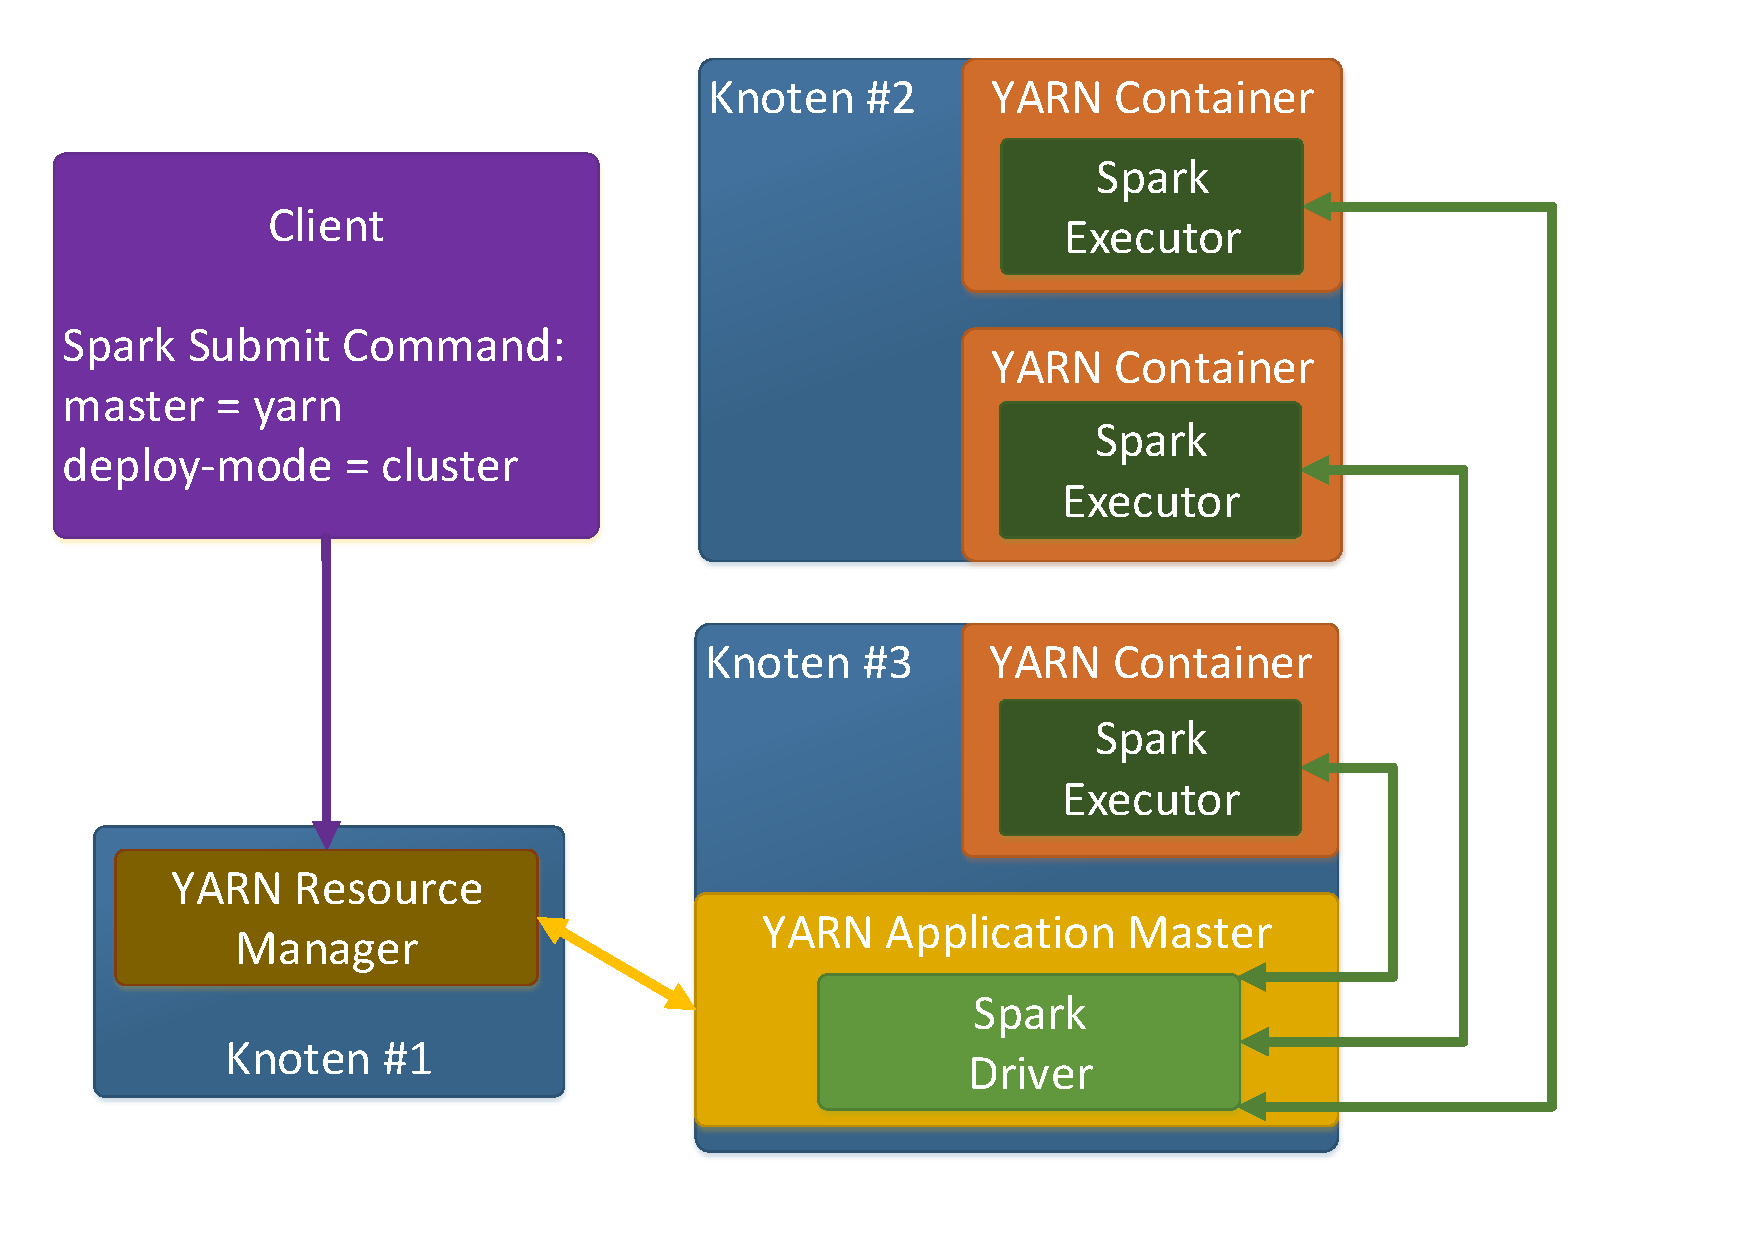
\includegraphics[width=\textwidth]{./resource/spark_cluster_architecture.pdf}
  \caption{Spark Datenverarbeitung im Cluster}
  \label{fig:spark_cluster_architecture}
\end{figure}

\noindent
Wie in Abbildung \ref{fig:spark_cluster_architecture} ersichtlich, wird die Ausführung einer Spark-Anwendung über den YARN-Ressourcenmanager gestartet. Es gibt hierbei unterschiedliche Wege, wie eine Spark-Anwendung ausgeführt werden kann. Im konkreten Fall wird das \textit{Spark-Submit} Kommando genutzt. Letztlich handelt es sich hierbei um einen Konsolenbefehl, welcher die Anwendung\footnote{Beispielsweise ist dies bei einer Spark-Anwendung in Java ein herkömmliches \textit{Java Archiv} im \textit{JAR}-Dateiformat.} selbst entgegennimmt und über diverse Parameter konfiguriert werden kann. So kann unter anderem der Master und Deploy Mode so konfiguriert werden, dass YARN die Ressourcen der Applikation verwaltet. Wie in Abbildung \ref{fig:yarn_cluster_architecture} (siehe Kapitel \ref{sec:theory_yarn}) bereits beschrieben, wird bei YARN ein ein Application Master erstellt, welcher wiederum diverse Ausführungscontainer auf den einzelnen Knoten anfordert und dieser überwacht. Bei der Ausfürung einer Spark-Anwendung werden diese Komponenten wiederverwendet und kapseln letztlich die falchlichen Komponenten von Spark.\\
So gibt es bei Spark einen sogenannten \textit{Driver}, welcher im Yarn Application Master läuft und wiederum die sogenannten \textit{Executor} aussteuert. Diese laufen wiederum gekapselt in einzelnen YARN Containern auf den Knoten. Ein Spark Executor entspricht aus Betriebssystemsicht eines Knotens im Cluster der Ausführung einer Java Virtual Machine (JVM) in einem eigenständigen Prozess. Aufgrund der Kapselung durch YARN können die einzelnen JVM-Prozesse überwacht werden und zur Not auch beendet werden, falls sie zu viel Ressourcen auf den Knoten anfordern.\\

\noindent
Hierzu muss Spark und YARN aber entsprechend konfiguriert werden, damit die Anwendungen auch korrekt im Cluster skaliert werden können. Nachfolgende Beispiel zeigt hier Konfigurationsmöglichkeiten.\\
Bei YARN und auch Spark beziehen sich die Ressourcen auf die Anzahl der genutzten CPU-Cores\footnote{Hierbei geht es um die virtuell verfügbaren CPU-Cores. So verfügt beispielsweise eine Intel CPU mit vier physikalischen Cores und Hyperthreading über insgesamt 8 virtuelle Cores zur parallelen Ausführung von Prozessen.} und die Größe des genutzten Arbeitsspeichers.\\

\noindent
\textbf{TODO}: Configurations Parameter in Cluster!\\

\noindent
Gerade wenn YARN einzelne Application-Container stoppt, weil sie zu viel Arbeitsspeicher benötigen deutet dies auf eine falsche Konfiguration oder falsche Programmierung der Spark-Anwendungen hin. Oftmals wird gerne der nutzbare Arbeitsspeicher pro Executor höher konfiguriert. Diese ist in den meisten Fällen jedoch der falsche Ansatz, da hierdurch kritische Probleme in der Programmlogik der Anwendung oftmals  nur kaschiert werden.\\ Daher ist es auf jeden Fall auch sinnvoll bei der Anwendungsentwicklung relativ kleine Cluster mit geringen Ressourcen zu nutzen, denn auch dort müssen die Anwendungen fehlerfrei ausführbar sein. Lediglich die Ausführungsgeschwindigkeit sollte sich in kleinen Clustern verlangsamen.\\ 
Aus diesem Grund werden im Rahmen dieser Thesis auch die Spark-Anwendungen auf einem einzelnen Knoten getestet, um Programmfehler besser und frühzeitiger erkennen zu können.\\
Einzelheiten zu den Programmierparadigmen und den grundlegenden Datenstrukturen können
in Kapitel \ref{ch:data_processing} nachgelesen werden.


\section{Apache HBASE}
\label{sec:theory_hbase}
\textit{Apache HBASE\textsuperscript{\textregistered}} ist eine spaltenorientierte \textit{NoSQL}-Datenbank. Sie entstand auf den Grundlagen der \textit{BigTable}-Datenbank von Google und wurde für das Speichern von Daten im Hadoop-Umfeld entwickelt.\footnote{Der Name \textit{HBASE} basiert auf der Kombination von \textit{Hadoop} und \textit{Database}.}\\
Der Begriff \textit{NoSQL}-Datenbank steht hierbei für \textit{Not only SQL} und beschreibt letztlich Datenbanken, welche Daten vorwiegend nicht in herkömmlichen relationalen Datenbankschemata speichern. Größtenteils sind diese Datenbanken schemafrei und können horizontal skaliert werden. Diese Bedingungen sind optimal zur Speicherung großer unstrukturierter Datenmengen.\\
Anhand des sogenannten \textit{CAP-Theorems} können diese Datenbanken kategorisiert werden.
Das CAP-Theorem besteht aus den Eigenschaften Konsistenz, Verfügbarkeit und Partitionstoleranz und besagt, dass maximal zwei dieser drei Eigenschaften von einer Datenbank garantiert werden können. Konsistenz beschreibt hier die Garantie, dass alle Knoten im verteilten System den gleichen Datenstand haben. Die Verfügbarkeit bezieht sich auf die dauerhafte Erreichbarkeit der Daten. Wohingegen die Partitionstoleranz die Funktionsfähigkeit selbst bei Ausfall einzelner Knoten im Datenbank-Verbundsystem garantiert.
Apache HBASE garantiert hierbei die Eigenschaften der Partitionstoleranz und der Konsistenz. Dies führt dazu, dass die Verfügbarkeit der Daten weniger stark ausgeprägt ist.
\cite[S. 189 ff.]{big_data_praxis}\\
% Vielleicht wäre auch hier eine Überlegung die Datenbank Cassandra zu nutzen, welche die Verfügbarkeit und Partitionstoleranz garantiert. An sich genommen ist die Konsistenz der Ergebnisse in der Forensik schon wichtig, allerdings sind nach der ersten Datenalyse eigentlich keine Änderungen auf den existierenden Datensätzen zu erwarten. Vielleicht wäre dann die Konsistenzgarantie ein Stück weit überflüssig und Cassandra könnte bessere Performanz bieten?

\noindent
Während herkömmliche relationale Datenbanken die Daten zeilenweise speichern, werden in spaltentorientierten Datenbanken die Daten spaltenweise gespeichert. Hierbei werden die Daten der einzelnen Spalten gruppiert in sogenannten \textit{Column Families} abgespeichert. Der Vorteil dieser Speicherart hängt stark von deren fachlichen Nutzung ab. Wenn alle Daten einer Spalte abgefragt werden, dann können diese Daten effizienter gelesen werden da sie zusammen persistiert wurden. Bei einer relationalen Datenbank hingegen wird bei solchen Anfragen die ganze Zeile mit allen Feldern gelesen, obwohl nur ein kleiner Teil dieser Daten wirklich benötigt wird.\\
%\textbf{TODO}: prüfen ob das so wirklich stimmt. Zumindest müssen einzelne Felder übersprungen werden, was ja nach Speicherart auch Zeit kostet.\\

\noindent
Apache HBASE basiert eben auf dieser Spaltenorientierung. Die Datenbank wird im Rahmen dieser Thesis für das Speichern beliebiger Dateiinhalte und Dateimetadaten verwendet. Ein vereinfachtes Beispiel einer möglichen Datenstruktur wird in Abbildung \ref{fig:hbase_schema_example} dargestellt.\\

\begin{figure}[ht]
  \centering
  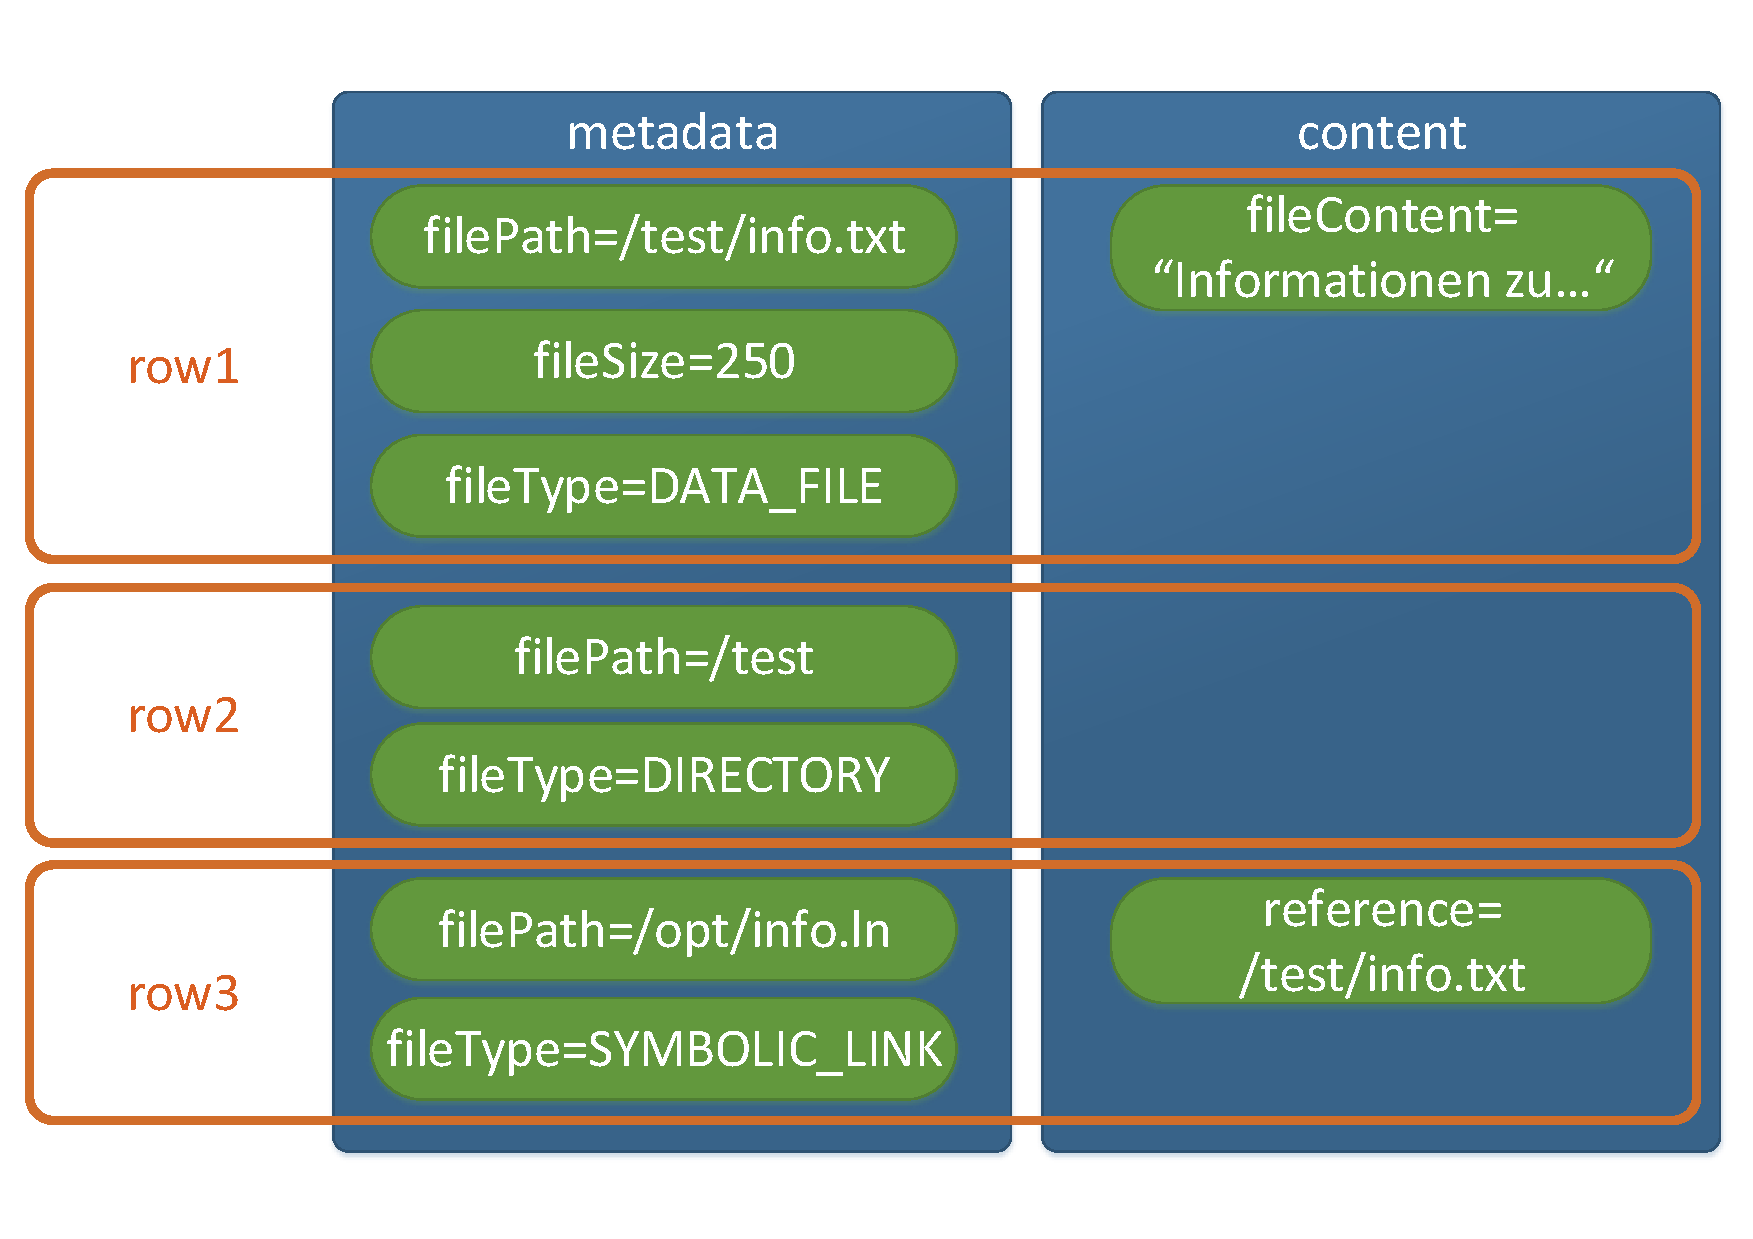
\includegraphics[width=0.8\textwidth]{./resource/hbase_data_schema_example.pdf}
  \caption{Schema-Beispiel einer HBASE Tabelle nach \cite{big_data_praxis}}
  \label{fig:hbase_schema_example}
\end{figure}

\noindent
Anhand der Abbildung werden einige Eigenschaften von HBASE sichtbar. So existieren zwei \textit{Column Families} mit den Namen \textit{metadata} und \textit{content}. Die Column Family \textit{metadata} enthält wiederum die Spalten \textit{filePath}, \textit{fileSize}und \textit{fileType}. Die Werte werden alle als Binär-Inhalt gespeichert. Eine Zeile hat dann jeweils einen eindeutigen Spaltenschlüssel, wie zum Beispiel \textit{row1}. 
Über diesen Schlüssel können die spezifischen Inhalte der einzelnen Spalten für eine bestimmte Zeile erfragt werden. Interessant hierbei ist, dass die Spaltenwerte optional sind und nicht für jede Zeile existieren müssen. So hat beispielsweise eine Datendatei, einen konkreten Inhalt, welcher in der Spalte \textit{fileContent} der Spaltenfamilie \textit{content} gespeichert werden. Ein Verzeichnis hingegen hat keinen Dateiinhalt. Daher ist in der zweiten Zeile auch kein Inhalt in der Spalte \textit{fileContent} abgelegt. In der dritten Zeile hingegen, wird ein symbolischer Link gespeichert. Dieser wiederum hat auch keinen Inhalt in der Spalte \textit{fileContent}. Dafür wird aber die Referenz auf die Originaldatei in einer weiteren Spalte gespeichert. Aufgrund der Gruppierung und Speicherung in Column Families benötigen leere Spaltenwerte auch keinen Speicherplatz. 
Ein einzelne Zelle beschreibt letztlich den Wert einer Spalte für eine konkrete Zeile. Hierbei wird zu jeder Zelle auch ein Zeitstempel gespeichert. Mithilfe diesen Zeitstempels können auch ältere Werte einer Zelle ausgelesen werden. 
So wird bei einer Modifikation einer konkreten Zelle der Wert inklusive eines neuen Zeitstempels geschrieben. Es ist jedoch immer noch möglich, ältere Zustände der Zelle zu lesen.\\
Aus Nutzersicht von Vorteil ist, dass die einzelnen konkreten Spalten innerhalb einer Spaltenfamilie nicht schon bei der Erstellung einer Tabelle angegeben werden müssen. Lediglich die Spaltenfamilien müssen initial angegeben werden und können später auch nicht mehr geändert werden. Somit kann nachträglich die Tabelle um weitere Spalten erweitert werden.\cite[S. 577]{hadoop_definitive_guide}\\

\noindent
Die Skalierbarkeit und die Partitionstoleranz wurden bei der Entwicklung von HBASE berücksichtigt. Es baut auf dem Hadoop HDFS auf und speichert darin die Daten. Analog zu HDFS, YARN oder Spark existiert auch hierbei eine Master-Slave Archtitektur über alle Knoten hinweg. Abbildung \ref{fig:hbase_cluster_architecture} zeigt die physikalische Aufteilung.\\

\begin{figure}[ht]
  \centering
  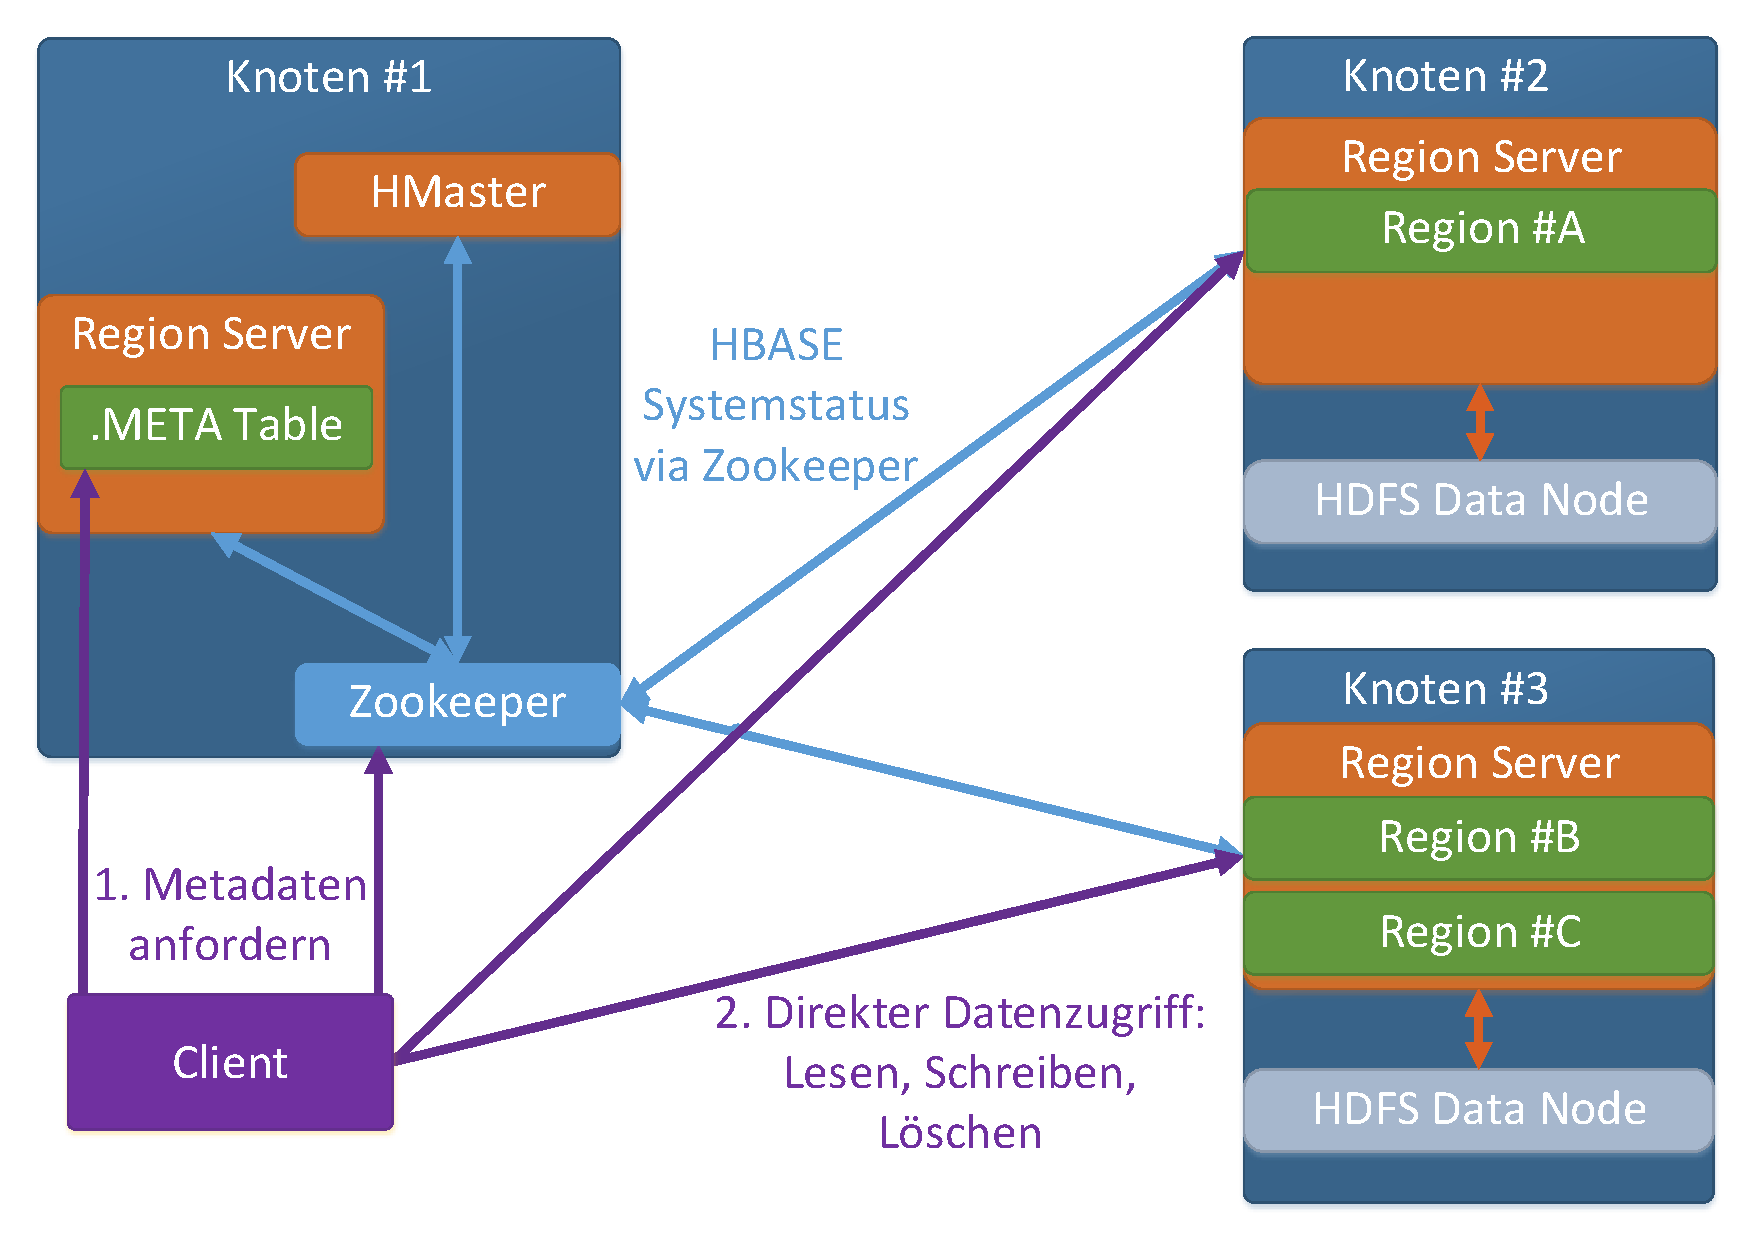
\includegraphics[width=\textwidth]{./resource/hbase_cluster_architecture.pdf}
  \caption{HBASE Datenspeicherung im Cluster}
  \label{fig:hbase_cluster_architecture}
\end{figure}

\noindent
Auf den einzelnen Knoten im Computer-Cluster laufen sogenannte \textit{Region Server}. Diese Region Server speichern jeweils unterschiedliche Teile der in HBASE angelegten Tabellen. Eine Tabelle selbst wird hierbei anhand der Zeilenschlüssel in mehrere Bereiche, den sogenannten \textit{Regions} unterteilt. Beispielsweise könnte die Region A (siehe Abbildung \ref{fig:hbase_cluster_architecture}) alle Daten einer Tabelle der Zeilen 1 bis 3000 enthalten. Die Region B wiederum enthält alle Daten der gleichen Tabelle aber von den Zeilen 3001 bis 8540. Und die Region C könnte die Daten der Zeilen 1 bis 22300 von einer anderen Tabelle enthalten. Somit kann ein Region Server mehrere Regions von gleichen oder auch unterschiedlichen Tabellen verwalten.  Das Prinzip der Datenlokalität greift auch bei HBASE. So sollte auf  jedem Knoten, auf dem ein RegionServer läuft, auch ein HDFS Data Node existieren. Dieser speichert die Daten der einzelnen Regions als Dateien im HDFS.\\

\noindent
Wenn neue Tabellen erstellt werden, oder einzelne Regions zu groß werden, dann koordiniert eine übergeordnete Instanz die Umverteilung von Daten und die Erstellung neuer Regions. Diese Instanz ist bei HBASE der sogenannte \textit{HMaster}. Es ist ein leichgewichtiger Prozess, welcher auf einem beliebigen Knoten im Cluster läuft und über Apache ZooKeeper auch den Status der einzelnen Region Server überwacht.\footnote{Die Funktionsweise von Apache ZooKeeper wird in Kapitel \ref{sec:theory_zookeeper} näher erläutert.}. Um die Ausfallsicherheit zu gewährleisten ist auch dieser Prozess redundant ausgelegt.\footnote{Über ZooKeeper kann immer der primäre HMASTER-Prozess ermittelt werden. Ist der aktive HMaster nicht mehr erreichbar, schaltet sich sich ein Backup-HMaster ein.} Darüber hinaus kümmert sich der HMaster-Prozess auch um die Restrukturierung bei Teilausfällen einzelner Region Server. 

\noindent
Wenn nun ein Client auf die Daten einer Tabelle zugreifen möchte, muss dieser wissen, auf welchem Knoten die Daten abgelegt sind. Hierfür verbindet sich der Client zuerst mit ZooKeeper und erfährt hierüber, welcher Region Server die sogenannte \textit{Meta-Tabelle} speichert.\cite[S. 579]{hadoop_definitive_guide}\\
Diese Meta-Tabelle enthält Informationen über alle Tabellen in HBASE inklusive der Region-Server und deren Regions die sie bereitstellen. Anhand dieser Metadaten kann der Client dann direkt die benötigten Daten an den entsprechenden Region Servern anfordern.\\
Dieses Vorgehen scheint für den Zugriff auf wenige Daten etwas aufwendig. Es skaliert aber sehr gut bei großen Datenmengen, da kein Flaschenhals vorhanden ist. Normalerweise speichert der Client die angeforderte Meta-Tabelle temporär, so dass er bei nachfolgenden Anfragen direkt au die entsprechenden Region Server zugreifen kann.\\ 

\noindent
Im Rahmen dieser Thesis wird HBASE beispielsweise verwendet um Metadaten zu speichern. Diese werden wiederum mit Apache Spark ausgelesen und verarbeitet. Hierbei kann das Prinzip der Datenlokalität sehr gut genutzt werden. Denn in der Theorie ist es durchaus möglich die HDFS Data Nodes, die Spark Worker und die HBASE Region Server getrennt auf unterschiedlichen Knoten auszuführen. Aber gerade dies macht keinen Sinn, da sonst immer wieder Daten über das Netzwerk transportiert werden müssen und dieses dann zum Flaschenhals der Verarbeitung wird.\\
Sinnvoll ist es nämlich HDFS Data Nodes auf den Knoten auszuführen, wo auch die Region Server ausgeführt. Darauf aufbauend sollten dann gerade auch die Spark Worker auf den Knoten die Datenverarbeitung ausführen, auf welchen die Region Server laufen. Dadurch können im besten Fall die Daten, welche durch Apache Spark benötigt werden, direkt von dem lokalen HBASE Region Server bereitgestellt werden. Dieser erhält die Daten wiederum von dem lokal laufendem Data Node. Somit können die Daten direkt auf dem Knoten verarbeitet werden, wo sie auch gespeichert sind und müssen nicht über das Netzwerk an andere Knoten gesendet werden.\footnote{Sie auch Kapitel \ref{sec:theory_yarn} und Kapitel \ref{sec:theory_spark}.} Die Koordinierung ist aber entsprechend komplex und viel wichtiger ist noch, dass jede einzelne Implementierung zur Prozessierung der Daten auch das Prinzip der Datenlokalität unterstützt.\\

\noindent
TODO: Erstellung eines adäquaten Zeilenschlüssels und dessen Auswirkungen (numerische Sortiertung, Hot Spot, ...) -> Dies könnte aber dann in Kapitel 4 oder 5 beschrieben werden!


\section{Apache ZooKeeper}
\label{sec:theory_zookeeper}

Innerhalb eines Computer-Clusters zur verteilten Datenverarbeitung existiert oftmals das Problem, dass sich die einzelnen Komponenten koordinieren müssen. Beispielsweise teilt HBASE die Daten auf mehrere RegionServer auf, welche wiederum auf den einzelnen Knoten laufen. Doch welche Instanz koordiniert diese Aufteilung? Ein anderes Problem ist der Datenzugriff. Ein Client möchte eine Zeile einer bestimmten Tabelle auslesen. Woher weiß der Client, welchen konkreten Knoten er anfragen muss, um genau diese Zeile zu erhalten? In den meisten Fällen existiert hierzu eine bestimmte Instanz, welche die Koordinierung der Knoten übernimmt. Beispielsweise gibt es bei HBASE den HMaster, welcher die Koordinierung übernimmt. Das Problem ist hierbei, dass auch der Knoten auf dem diese Master-Instanz läuft ausfallen kann und das komplette System zum erliegen bringt. Diese Master-Instanzen im allgemeinen sind kritische Komponenten und können als Single-Point-of-Failure zu einem Stillstand des kompletten Systems führen. Um solche Totalausfälle zur vermeiden, müssen bestimmte Automatismen definiert werden, wie sich die Knoten selbst organisieren können, um einen Ausfall beliebiger Knoten zu überstehen.\\

\noindent
An dieser Stelle bietet \textit{Apache ZooKeeper\texttrademark\thinspace} Mechanismen an, wie sich die einzelnen Knoten in einem verteilten System organisieren und Informationen verteilt synchronisieren können. Aus logischer Sicht stellt ZooKeeper einen Service zu Verfügung. Dieser Service ermöglicht das Speichern von Informationen strukturiert als Verzeichnis mit einzelnen Dateien. Bei den Informationen handelt sich normalerweise um wichtige Konfigurationen, welche im Cluster verteilt werden müssen und zentral über ZooKeeper aktualisiert werden können. Jeder Client, der sich mit ZooKeeper innerhalb des Computer-Clusters verbindet, sieht die gleiche Konfiguration und kann bei Bedarf auch bestimmte Konfigurationen ändern.\cite[S. 4 ff]{professional_hadoop} \\
Aus Sicht des Entwicklers, stellt dieser Service immer die aktuellen Informationen im Cluster zu Verfügung. Wie der Service dies bewerkstelligt ist ein Implementierungs-Detail. Neben dem bereits erwähnten Konfigurationsmanagement bietet ZooKeeper auch einen Naming-Service oder auch die Möglichkeit den Live-Status einzelner Knoten zu überwachen.\cite{zookeeper_essentials}\\
Wie bei HBASE in Kapitel \ref{sec:theory_hbase} bereits erwähnt, kann ein Client sich mit ZooKeeper verbinden und erhält über ZooKeeper den aktuellen Knoten, welcher die Metadaten zu allen Tabellen in HBASE Speichert. Ein anderes Beispiel zeigt die Backup-Instanz des HMaster-Prozesses. Dieser prüft über ZooKeeper den Status des primären HMaster-Prozesses und wird informiert, wenn letzterer nicht mehr verfügbar ist. Daraufhin propagiert sich die Backup-Instanz als neuen HMaster-Prozess im Cluster, um so die Funktionsfähigkeit von HBASE aufrecht zu erhalten. Abbildung \ref{fig:zookeeper_dir} zeigt die Verzeichnisstruktur, welche stark an ein Unix-Verzeichnis erinnert. Wobei die einzelnen Einträge sogenannten \textit{ZNodes} entsprechen.\footnote{Siehe auch \url{http://zookeeper.apache.org/doc/r3.5.4-beta/zookeeperOver.html}, Stand: 26.7.2018} \\

\begin{figure}[ht]
  \centering
  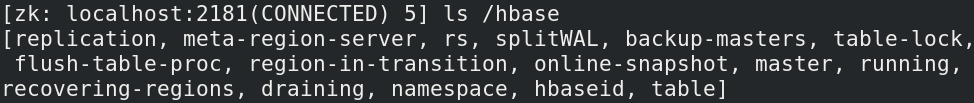
\includegraphics[width=\textwidth]{./resource/zookeeper_dir.png}
  \caption{Gespeicherte Informationen von HBASE in ZooKeeper}
  \label{fig:zookeeper_dir}
\end{figure}


\noindent
Normalerweise ist Zookeeper auf mehreren Knoten im Cluster installiert. Sie bilden ein sogenanntes \textit{ZooKeeper Ensemble} und bestehen zumeist aus 3 oder 5 Einzelinstallationen auf beliebigen Knoten. Ein ZooKeeper Ensemble, welches für die gleiche Anwendungsdomäne zuständig ist, wird auch \textit{Quorum} genannt. Innerhalb eines Quorums gibt es einen Leader und mehrere Follower, die sich die gleichen Konfigurationsinformation teilen. Fällt der Leader aus, können die Follower einen neuen Leader bestimmen.\cite{zookeeper_essentials}\\

\section{Apache Solr}
\label{sec:theory_solr}